\PassOptionsToPackage{table,dvipsnames,svgnames}{xcolor}
\documentclass[portrait,final,a0paper]{nadiposter}

\usepackage{fontawesome}

\selectcolormodel{RGB}

\usepackage{graphicx}
\usepackage{multicol}
\usepackage{sectsty}


\usepackage{pgfbaselayers}
\pgfdeclarelayer{background}
\pgfdeclarelayer{foreground}
\pgfsetlayers{background,main,foreground}


%%%%%%%%%%%%%%%%%%%%%%%%%%%%%%%%%%%%%%%%%%%%%%%%%%%%%%%%%%%%%%%%%%%%%%%%%%%%%%%%
% Multicol Settings

\setlength{\columnsep}{1.5em}
\setlength{\columnseprule}{0mm}

%%%%%%%%%%%%%%%%%%%%%%%%%%%%%%%%%%%%%%%%%%%%%%%%%%%%%%%%%%%%%%%%%%%%%%%%%%%%%%%%


% ----------------------------------------------------------------------- %

% Useful hints
% https://tex.stackexchange.com/questions/252757/including-boxes-inside-boxes-in-baposter

% ----------------------------------------------------------------------- %



\newcommand{\compresslist}{%
\setlength{\itemsep}{1pt}%
\setlength{\parskip}{0pt}%
\setlength{\parsep}{0pt}%
\setlength{\leftmargin}{0pt}%
}


\contactInfo{%
\begin{tabular}{c}
  Jean-Marie Jacquet \\
  \faEnvelopeO\ : jean-marie.jacquet@unamur.be \\
  \faGlobe\ : staff.info.unamur.be/jmj
\end{tabular}}



\begin{document}

\definecolor{unamurgreen}{RGB}{69,181,63}
\definecolor{unamurgray}{RGB}{64,68,67}
\definecolor{lightunamurgreen}{RGB}{69,181,63}

% from poster example

\definecolor{lightorange}{rgb}{0.9,0.4,0}
\definecolor{lightestorange}{rgb}{1,0.8,0.5}
\definecolor{darkorange}{rgb}{0.2,0.1,0}

% end from poster example


\typeout{Poster Starts}


\begin{poster}%
  % Poster Options
  {
  % Show grid to help with alignment
  % grid=true,
  grid=false,
  % Column spacing
  colspacing=1em,
  % Color style
  bgColorOne=lightunamurgreen,
  bgColorTwo=white,
  borderColor=unamurgray,
  headerColorOne=unamurgray,
  headerColorTwo=lightorange,
  headerFontColor=white,
  boxColorOne=white,
  boxColorTwo=white,
  % Format of textbox
  textborder=roundedright,
  % Format of text header
  eyecatcher=true,
  headerborder=closed,
  headerheight=0.1\textheight,
%  textfont=\sc, An example of changing the text font
  headershape=roundedleft,
  headershade=plain,
  headerfont=\Large\bf\textsc, %Sans Serif
  textfont={\setlength{\parindent}{1.5em}},
  boxshade=plain,
  background=plain,
  linewidth=2pt,
  columns=4
  }
  % Eye Catcher
  {\hbox{} } %
\includegraphics[height=7em]{images/nadi-red.png}} 
  % Title
  {\bf\textsc{The Joy of Declarative and \\*[0.3em] Concurrent Programming}\vspace{0.5em}}
  % Authors
  {\textsc{Jean-Marie Jacquet -- CoordiNam Lab} }
  % University logo
  {% The makebox allows the title to flow into the logo, this is a hack because of the L shaped logo.
   \hbox{} % 
\includegraphics[height=7em]{images/nadi-red.png}
  }


% --------------------------------------------------------------------------- %

\sectionfont{\centering}

\headerbox{Concurrent logic programming}{name=clp,column=0,row=0,span=3}{

\begin{multicols}{2}

\section*{The framework}

\( \begin{array}{l}
grand\_parent(X,Y) \leftarrow parent(X,Z), parent(Z,Y) \\
parent(jules,marie) \\
parent(marie,antoine) \\ % \\*[0.5em]
?- grand\_parent(jules,C)
\end{array}
\)

\section*{Issues}


\begin{itemize}
\compresslist

\item Concurrency (evaluate in parallel)
\item Constraints (equality $\rightarrow$ constraints)
\item Contextual programming (handle contexts)

\end{itemize}

\section*{Applications}

\begin{itemize}
\compresslist

\item Casubel : expert system in estate planning
\item Expesurf : expert system in multi-layer surface engineering
\item BEM : business event manager

\end{itemize}

\bigskip
\begin{center}

\includegraphics[height=3em]{images/casubel.png}
\end{center}

\end{multicols}
}


\newcommand{\mgoal}[1]{\overline{#1}}
\newcommand{\decl}[1]{\mbox{$\; \models_{\mbox{\scriptsize {#1}}} \;$}}
\newcommand{\cl}{\mbox{$\leftarrow$}}
\newcommand{\mf}[1]{\mbox{#1}}
\newcommand{\tpd}{\mbox{$ \; \vdash \; $}}
\newcommand{\fiden}{\mbox{$\Psi_{den}$}}
\newcommand{\fip}{\mbox{$\Psi_{\parallel}$}}
\newcommand{\parop}{\mbox{ $ \tilde{\parallel} $ }}

\sectionfont{\raggedright}

\headerbox{Semantics}{name=semantics,column=3,row=0,span=1}{


\section*{Declarative}

\( \begin{array}{l}
S \decl{I} A \mbox{ iff } A \in S \\
S \decl{I} (H \cl \mgoal{B}) \mbox{ iff } \\
\hspace*{5ex} S \decl{I} H \mbox{ whenever } S \decl{I} \mgoal{B} \\
\end{array} \)

\section*{Operational}

\( \begin{array}{l}
%
\frac{ \mf{P} \tpd \mf{A}_{1} \; [\theta_{1}], \; \cdots, \;  
       \mf{P} \tpd \mf{A}_{m} \; [\theta_{m}]
    }{ \mf{P} \tpd \mf{A}_{1},\ldots,\mf{A}_{m}
            \; [\rho(\theta_{1},\ldots,\theta_{m})]
     }
\\ \\
\frac{ \mf{P} \tpd \mgoal{B}\theta \; [\sigma]
    }{ \mf{P} \tpd \mf{A} \;[\theta\sigma]
    }
\hspace*{2ex}\mbox{ if }
   \left\{ \begin{array}{l}
       (\mf{H}\leftarrow\mgoal{B}) \in \mf{P} \\
       \theta = \mf{mgu(A,H)}
       \end{array}\right.
\\*[1em]
\langle A,\epsilon \rangle \longrightarrow
   \langle \mgoal{B_1},\theta_1 \rangle \longrightarrow \cdots
\end{array} \)


\section*{Denotational}

\( \begin{array}{l}
     \fiden (\mf{F}) (\mf{P}) ( (A_{1},\cdots,A_{m})(\sigma) )
     = \\ \hspace*{1ex} 
     \fiden (\mf{F}) (\mf{P}) (A_{1})(\sigma)  
     \parop
     \cdots
     \parop \mbox{ } \\ \hspace*{1ex}
     \fiden (\mf{F}) (\mf{P}) (A_{m})(\sigma)
     \\ \cdots
     \\
     \fip(\mf{F})(\mf{p}_{1},\mf{p}_{2}) = \\ \hspace*{1ex}
        \{ (\omega,\mf{F}(\mf{p'$_{1}$},\mf{p'$_{2}$})) : \cdots \} \cup \cdots \mbox{ }
%         \cup
%         \{ (\omega,\mf{F}(\mf{p'$_{1}$},\mf{p$_{2}$})) : \cdots F \cdots \}
%        \cup    
%        \{ ( \omega,\mf{F}(\mf{p$_{1}$},\mf{p'$_{2}$}) ) : \cdots F \cdots \}
\end{array} \)


\begin{center}
\textit{\textcolor{red}{Completely different semantics than
for classical concurrency}}
\end{center}


}



\newcommand{\seqcc}[2]{ {#1} \; ; \; {#2} }
\newcommand{\paracc}[2]{ {#1} \; || \; {#2} }
\newcommand{\choicecc}[2]{ {#1} \; + \; {#2} }

\newcommand{\choicec}{ +  }

\newcommand{\bset}{ \{ }
\newcommand{\eset}{ \} }
\def\Scvar{\mathit{Scvar}}
\def\Sstring{\mathit{Sstring}}
\def\Scpterm{\mathit{Scpterm}}

\newcommand{\conf}[2]{ {<} {#1}, {#2} {>} }
\newcommand{\trans}[2]{ {#1} \longrightarrow {#2} }
\newcommand{\transm}[2]{ {#1} \longrightarrow {#2} } 

\newcommand{\bmset}{ \{ }
\newcommand{\emset}{ \} }

\newcommand{\infrule}[2]{%
 \begin{array}{c}
       {#1} \\
       \hline
       {#2}
\end{array}
}


\headerbox{Coordination languages and models}{name=coord,column=0,span=3,below=clp}{

\section*{BachT, the basic model}

\begin{multicols}{2}

\begin{center}

\setlength{\unitlength}{0.4cm}
\begin{picture}(14,9)(0,1)

\put(7,5){\oval(6,4.5)}

\put(1,9){\makebox(0,0){$P$}}
\put(1,1){\makebox(0,0){$R$}}

\put(13,9){\makebox(0,0){$Q$}}
\put(13,1){\makebox(0,0){$S$}}

\put(1.6,8.8){\vector(3,-2){2.2}}
\put(1.6,1.2){\vector(3,2){2.2}}

\put(12.4,8.8){\vector(-3,-2){2.2}}
\put(12.4,1.2){\vector(-3,2){2.2}}

\put(2.8,8.4){\makebox(0,0)[bl]{{\small $tell(t)$}}}
\put(2.8,1.6){\makebox(0,0)[tl]{{\small $nask(t)$}}}

\put(11.2,8.4){\makebox(0,0)[br]{{\small $ask(t)$}}}
\put(11.2,1.6){\makebox(0,0)[tr]{{\small $get(t)$}}}

\end{picture}
\end{center}

\begin{eqnarray*}
    C   & ::= &   tell(t) \ | \ ask(t) \ | \ nask(t)  \ | \ get(t)
\\
    A   & ::= &   C \ | \ \seqcc{A}{A} \ | \
                  \paracc{A}{A} \ | \ \choicecc{A}{A}
\end{eqnarray*}

\medskip
\noindent
\textbf{\textit{Properties :}}
\begin{itemize}
\compresslist
\setlength{\topsep}{0pt}
\setlength{\partopsep}{0pt}%

\item associative memory
\item asynchronous communication
\item persistent broadcast communication
\item decoupling in space and time

\end{itemize}

\vspace*{1cm}
\( \begin{array}{l}
%
     \trans{ \conf{ tell(t) }{ \sigma }
          }{ \conf{ E }{ \sigma \cup \bmset t \emset }
           }
\\ 
     \trans{ \conf{ ask(t) }{ \sigma \cup \bmset t \emset }
          }{ \conf{ E }{ \sigma \cup \bmset t \emset }
           }
\\ 
     \trans{ \conf{ nask(t) }{ \sigma }
          }{ \conf{ E }{ \sigma }
           }
     \hspace*{2ex} \mbox{ for t }\not\in \sigma
\\ 
     \trans{ \conf{ get(t) }{ \sigma \cup \bmset t \emset }
          }{ \conf{ E }{ \sigma }
           }
\end{array} \)

\end{multicols}

\section*{Extensions}

\begin{multicols}{3}

\begin{itemize}
\compresslist

\item structured data and variables
\item processes as active data
\item time (relative and absolute)
\item multiplicity

\end{itemize}

\begin{itemize}
\compresslist

\item chemical abstraction
\item distribution
\item relations
\item mobility

\end{itemize}

\begin{center}
\begin{tabular}{c}
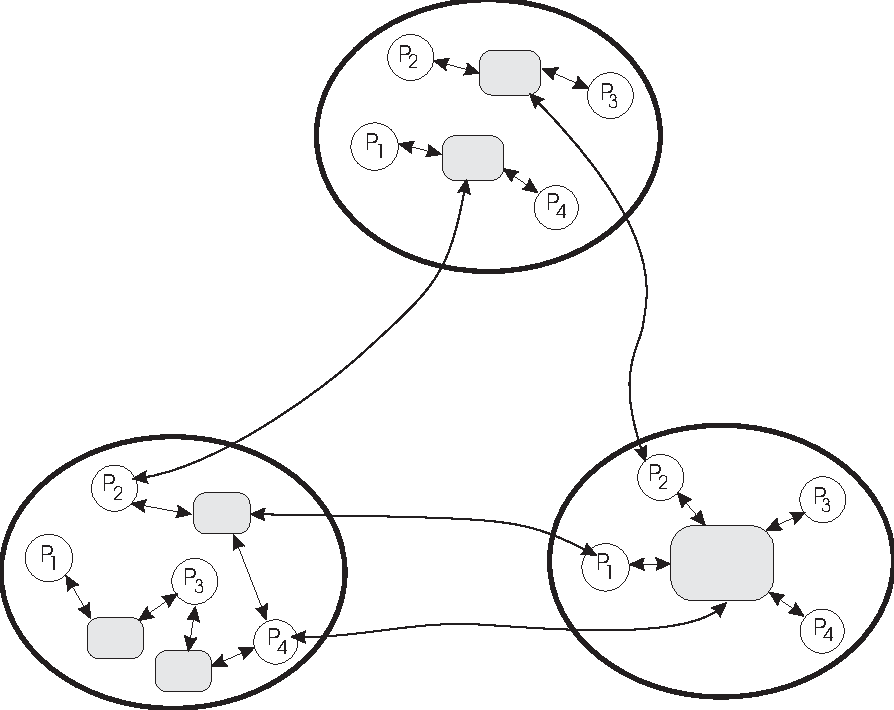
\includegraphics[height=5em]{images/mu2log.pdf} \\
No master manager
\end{tabular}
\end{center}



\end{multicols}

}

\headerbox{Expressiveness}{name=exp,column=3,span=1,below=semantics}{

\begin{center}
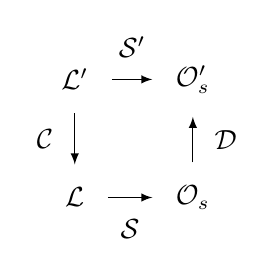
\begin{tikzpicture}

\node at (0,1.5) (Lprim) {${\mathcal L}'$};
\node at (0,0) (L)  {${\mathcal L}$};
\node at (1.5,1.5) (Oprim)  {${\cal O}'_{s}$};
\node at (1.5,0) (O)  {${\cal O}_{s}$};

\draw[-latex,shorten <=5pt,shorten >=5pt] (Lprim) -- node[left,xshift=-1ex] {${\cal C}$}  (L);
\draw[-latex,shorten <=5pt,shorten >=5pt] (Lprim) -- node[above,yshift=1ex] {${\cal S}'$} (Oprim);
\draw[-latex,shorten <=5pt,shorten >=5pt] (O) -- node[right,xshift=1ex] {${\cal D}$} (Oprim);
\draw[-latex,shorten <=5pt,shorten >=5pt] (L) -- node[below,yshift=-1ex] {${\cal S}$} (O) ; 

\end{tikzpicture}
\end{center}

\[ \begin{array}{l}
     {\cal L}(tell) \\ \mbox{ } < {\cal L}(tell,ask) 
       < {\cal L}(tell,get) \\ \mbox{ } < {\cal L}(tell,ask,get,nask)
   \end{array}
\]

}

\headerbox{Methodology}{name=future,column=3,span=1,below=exp}{

\begin{center}
\begin{tabular}{l}
Programming = \\*[0.5em] \hspace*{2ex} Computation + Coordination
\end{tabular}
\end{center}

\bigskip
\begin{itemize}
\compresslist

\item Code each component separately assuming data is available
\item Ensure required data is indeed available
\end{itemize}

}

\sectionfont{\centering}

\headerbox{Future work}{name=future,column=0,span=3,below=coord}{

\begin{multicols}{3}

\section*{Foundations}

\begin{itemize}
\compresslist

\item extensions (e.g. probability, relation and time, capacity)
\item programming environments
\item implementations
\item links with other models \\(e.g. Reo, mcrl2)
\item logics

\end{itemize}

\section*{Blockchain}

\begin{center}
\begin{tabular}{c}
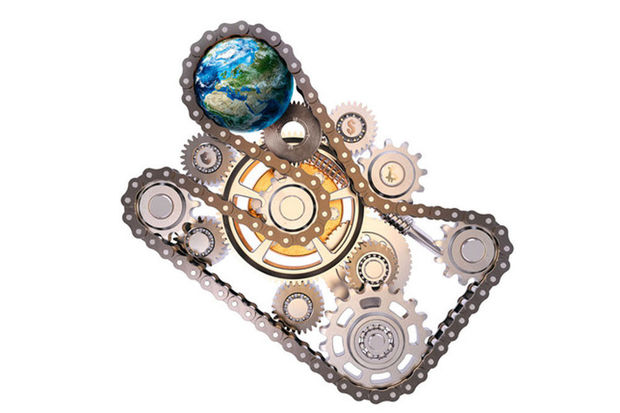
\includegraphics[height=5em]{images/blockchain.jpg}\\
(image DataNews (21/03/18)) \\
\end{tabular}
\end{center}

\begin{center}
How to coordinate modern distributed systems ? 
\end{center}


\section*{Bio-algorithmics}

\begin{center}
\begin{tabular}{c}
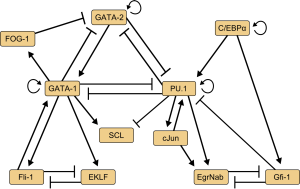
\includegraphics[height=5em]{images/gnr.png}\\
(image PLoS One 2011;6(8)) \\
\end{tabular}
\end{center}

\begin{center}
How to apply process algebra techniques ? 
\end{center}

\end{multicols}

}


\headerbox{Conclusion}{name=conc,column=0,span=4,below=future}{

\noindent
\begin{minipage}{0.65\linewidth}   
\begin{itemize}
\compresslist

\item Declarative and concurrent programming is fun and opens interesting research questions
\item The CoordiNam Lab offers expertise in functional and logic programming,
      concurrent programming,
      formal methods, and coordination languages
\item Part of this work has been made in collaboration with A. Brogi, D. Darquennes, K. de Bosschere,
      I. Linden, L. Monteiro 

\end{itemize}
\end{minipage}
\hfill
\begin{minipage}{0.35\linewidth}
\begin{flushright}
\begin{tabular}{cccc}

\includegraphics[height=6em]{images/lncs1.jpg} &

\includegraphics[height=6em]{images/rwiley2.jpeg}&

\includegraphics[height=6em]{images/lncs2.jpg} &

\includegraphics[height=6em]{images/lncs3.jpg} 
\end{tabular}
\end{flushright}
\end{minipage}
  
}

\end{poster}

\end{document}

